\documentclass[10pt,letterpaper]{article}

\usepackage{templates/cogsci}
\usepackage{natbib}
\usepackage{pslatex}
\usepackage{graphicx}
%% \usepackage{supertabular}
\usepackage{supertabular,booktabs}

%% Tighter grouping of figures.
\renewcommand{\textfraction}{0.15}
\renewcommand{\topfraction}{0.85}
\renewcommand{\bottomfraction}{0.70}
\renewcommand{\floatpagefraction}{0.66}


\title{Creating words from iterated vocal imitation}

\author{{\large \bf Pierce Edmiston (pedmiston@wisc.edu)} \\
  Department of Psychology, 1202 W. Johnson Street \\
  Madison, WI 53706 USA \\
  \AND {\large \bf Marcus Perlman (marcus.perlman@mpi.nl)} \\
  Max Planck Institute for Psycholinguistics \\ 
  Nijmegen, 6500 AH The Netherlands \\
  \AND {\large \bf Gary Lupyan (lupyan@wisc.edu)} \\
  Department of Psychology, 1202 W. Johnson Street \\
  Madison, WI 53706 USA}

\begin{document}

\maketitle

\begin{abstract}
We report the results of a large-scale (\emph{N} = 1571) experiment to
investigate whether spoken words can emerge from the process of repeated
imitation. Participants played a version of the children's game
``Telephone''. The first generation was asked to imitate recognizable
environmental sounds (e.g., glass breaking, water splashing); subsequent
generations imitated the imitators for a total of 8 generations. We then
examined whether the vocal imitations became more stable and word-like,
retained a resemblance to the original sound, and became more suitable
as learned category labels. The results showed (1) the imitations became
progressively more word-like, (2) even after 8 generations, they could
be matched above chance to the environmental sound that motivated them,
and (3) imitations from later generations were more effective as learned
category labels. These results show how repeated imitation can create
progressively more word-like forms while retaining a semblance of
iconicity.

\textbf{Keywords:}
categorization; transmission chain; language evolution

\end{abstract}

People have long pondered the origins of languages, especially the words
that compose them. For example, both Plato in his \emph{Cratylus}
dialogue \citep{Plato:1999uk} and John Locke in his \emph{Essay
Concerning Human Understanding} \citep{Locke:1948eu} examined the
``naturalness'' of words--whether they are somehow imitative of their
meaning. Some theories of language evolution have hypothesized that
vocal imitation played an important role in generating the first words
of spoken languages
\citep[e.g.,][]{Brown:1955wy, Donald:2016kd, Imai:2014dea, Perlman:2015ip};
early humans may originally have referred to a predatory cat by
imitating its roar, or to the discovery of a stream by imitating the
sound of rushing water. Such vocal imitation might have served to
clarify the referent of a vocalization and eventually establish a
mutually understood word. In this study, we investigate the formation of
onomatopoeic words--imitative words that resemble the sounds to which
they refer. We ask whether onomatopoeic words can be formed gradually
and without instruction simply from repeating the same imitation over
generations of speakers.

Onomatopoeic words appear to be a universal lexical category found
across the world's languages \citep{Dingemanse:2012fc}. Languages all
have conventional words for animal vocalizations and various
environmental sounds. \citet{Rhodes:1994au}, for example, documented a
repertoire of over 100 onomatopoeic words in English, which he notes
exist along a continuum from ``wild'' to ``tame''. People often use more
wild vocal imitations and other sound effects during demonstrative
discourse, especially when producing quotations
\citep{Blackwell:2015ix, Clark:1990cl}. Wild words have a more imitative
phonology whereas tame words take on more standard phonology of other
English words. In some cases, words that begin as wild imitations of
sounds become fully lexicalized and integrated into the broader
linguistic system, when they behave like more ``ordinary'' words that
can undergo typical morphological processes. Examples are English words
like ``crack'' or the recently adapted ``ping''.

\begin{figure}

{\centering 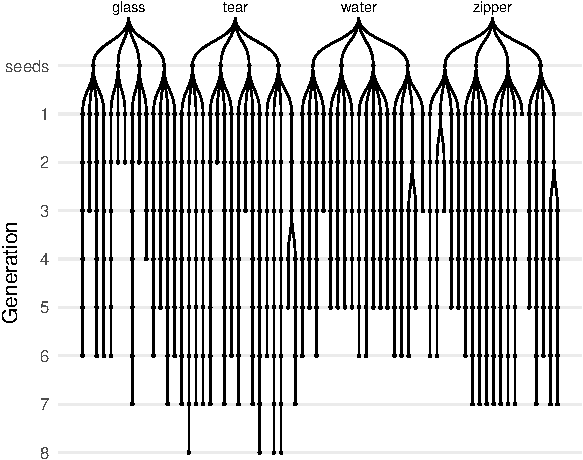
\includegraphics[width=5.0cm]{figs/fig1-1} 

}

\caption{The design of the transmission chain experiment. 16 seed sounds were selected, four in each category of environmental sounds. Participants imitated each seed sound, and then the next generation of participants imitated the imitations and so on for 8 generations.}\label{fig:fig1}
\end{figure}

However, not all researchers agree that vocal imitation has any
significant role in language. For instance, \citet{Pinker:2005cv}
suggested that, ``Humans are not notably talented at vocal imitation in
general, only at imitating speech sounds (and perhaps melodies). For
example, most humans lack the ability (found in some birds) to
convincingly reproduce environmental sounds \ldots{} Thus `capacity for
vocal imitation' in humans might be better described as a capacity to
learn to produce speech.'' Nevertheless, experiments show that people
can actually be quite effective at using vocal imitation. For example,
\citet{Lemaitre:2014kr} collected imitations and verbal descriptions of
various mechanical and synthesized sounds. When participants listened to
these and were asked to identify the source, they were more accurate
with imitations than descriptions. A subsequent study found that vocal
imitations tend to focus on a few salient features of the sound rather
than a high fidelity representation, which aids identification of the
source \citep{Lemaitre:2016kz}.

Thus humans can be effective at communicating with vocal imitation, it
can play an important role in narration and discourse, and it appears to
be the basis for substantial inventories of sound-imitative vocabulary
across languages. But the process by which onomatopoeic words like
``meow'', ``ping'' and ``buzz'' emerge from vocal imitations has yet to
be observed. Here we examine whether simple repeated imitations of
environmental sounds become more word-like even in the absence of
explicit communication intent or the intent to create a word-like token.
Alternatively, repeating imitations might never stabilize on a
particular wordform, or the limited fidelity of human vocal imitation
may simply restrict the formation of stable words through iterated
imitations.

To test this, we recruited participants to engage in a large scale
online version of the children's game of ``Telephone'' in which an
acoustic message is passed from one person to the next. After obtaining
these imitations, we investigated how the imitations changed over
generations to determine whether they became more word-like. We
investigated the acoustic properties of the imitations as well as the
orthographic properties once transcribed into English words. We find
that by both measures the imitations become more stable through
repetition. In addition to stability, we also find that the imitations
can still be matched back to the original sounds at above chance levels
for many generations. Finally, we measured how quickly the invented
words are learned as category labels in a category learning experiment,
and find that later generation imitations are easier to learn as
category labels.

\section{General Methods}\label{general-methods}

In Experiment 1 we collected iterated vocal imitations using the
transmission chain design depicted in Fig. 1. We then assessed changes
in these imitations over generations in the remaining experiments, which
are listed in Table 1. In Experiment 2 we assessed the extent to which
each imitation could be matched back to its originating sound.
Experiment 3 involved collecting transcriptions of imitations, and these
transcriptions were matched back to the original sounds in Experiment 4.
In Experiment 5 we selected transcriptions taken from first and last
generation imitations as novel labels in a simple category learning
experiment.

\begin{table}

\caption{\label{tab:table1}List of experiments and sample sizes. Participants in Experiments 1-4 were recruited via Amazon Mechanical Turk and paid to participate in an online study. Participants in Experiment 5 were University of Wisconsin-Madison undergraduates who received course credit in exchange for participation.}
\centering
\begin{tabular}[t]{rlr}
\toprule
\# & Experiment & N\\
\midrule
1 & Collecting imitations & 94\\
2 & Matching imitations to seeds & 752\\
3 & Collecting transcriptions & 218\\
4 & Matching transcriptions to seeds & 444\\
5 & Category learning & 63\\
\bottomrule
\end{tabular}
\end{table}

\section{Experiment 1: Collecting
imitations}\label{experiment-1-collecting-imitations}

In Experiment 1 we collected the iterated vocal imitations that served
as the basis for the remaining experiments. Our hypothesis was that
these vocal imitations would become more stable as they were repeated
over generations of speakers.

\subsection{Methods}\label{methods}

\subsubsection{Materials}\label{materials}

We initially selected a set of 36 sounds in 6 different categories of
environmental sounds. Inanimate categories of sounds were selected
because they were less likely to have lexicalized onomatopoeic forms
already in English, and they were assumed to be less familiar and more
difficult to imitate. We used an odd-one-out norming procedure (\emph{N}
= 105 participants) to reduce this initial set to 16 ``seed'' sounds: 4
sounds in each of 4 categories. The four final categories included:
water, glass, tear, zipper.

\subsubsection{Procedure}\label{procedure}

Participants were paid to participate in an online version of the
children's game of ``Telephone''. The instructions informed participants
that they would hear some sound and their task is to reproduce it as
accurately as possible using their computer microphone. Participants
listened to and imitated 4 sounds. Participants received one sound from
each of the four categories of sounds drawn at random such that
participants were unlikely to hear the same person more than once.

Imitations were monitored by an experimenter to catch any gross errors
in recording before they were passed on to the next generation of
imitators. The experimenter also blocked sounds that violated the rules
of the experiment, e.g., by saying something in English.

Given large differences in recording quality resulting from conducting
the experiment online, we were unable to use previously published
techniques for calculating acoustic distance
\citep[cf.][]{Lemaitre:2016kz}. Instead, we obtained subjective measures
of acoustic similarity using a controlled, randomized norming procedure
completed by research assistants. Five RAs listened to pairs of
imitations while blind to generation and rated their similarity on a
7-point scale where a 1 meant the sounds could never be confused with
one another and a 7 meant the sounds were nearly identical. Prior to
analysis, the similarity ratings were converted to z-scores for each
rater.

\subsection{Results}\label{results}

We collected a total of 480 imitations, of which 115 were removed,
leaving 365 imitations along 105 contiguous transmission chains for
analysis. Imitations from later generations were rated as being more
similar to one another than imitations from earlier generations,
\emph{b} = 0.10 (0.03), \emph{t}(3.5) = 3.86, \emph{p} = 0.026 (Fig. 2),
suggesting that the imitations are stabilizing through repetition.

\begin{figure}
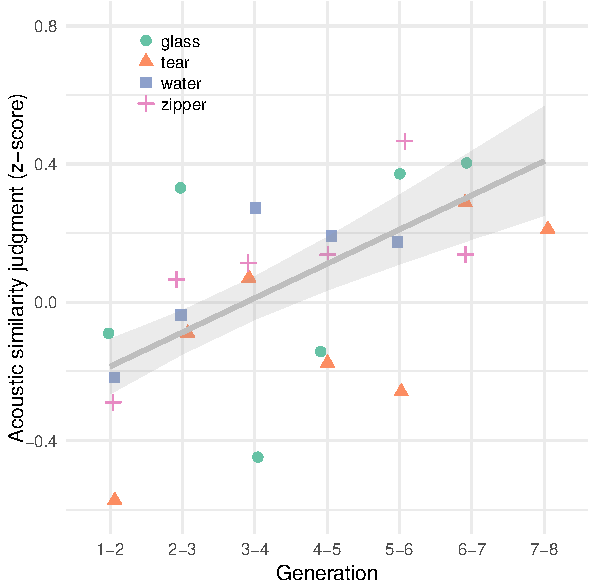
\includegraphics[width=8cm]{figs/fig2-1} \caption{Increase in acoustic similarity over generations. Points depict mean acoustic similarity ratings for imitations in each category of environmental sounds. The predictions of the linear mixed effects model with random effects for rater and category are shown, with error bands denoting +/- 1 standard error of the model predictions.}\label{fig:fig2}
\end{figure}

\section{Experiment 2: Matching imitations to
seeds}\label{experiment-2-matching-imitations-to-seeds}

Experiment 2 was conducted to determine if the imitations retained some
resemblance to the original environmental sound that motivated it
(i.e.~the seed sound). Participants completed a 4-alternative forced
choice test in which they heard an imitation and had to select which of
four possible sounds they thought the imitation most closely resembled.
By varying the relationship between the imitation and the four options
presented to each participant, we were able to assess the extent to
which the imitations retained categorical as opposed to specific,
identifying information. On the view that repetition makes the
imitations more word-like, we expected later imitations to be better
matched to categories of sounds as opposed to specific sounds within
each category.

\subsection{Methods}\label{methods-1}

\subsubsection{Materials}\label{materials-1}

All 365 imitations collected in Experiment 1 were tested in each
condition depicted in Fig. 3.

\subsubsection{Procedure}\label{procedure-1}

On each trial participants listened to an imitation and selected among
four possible options as to which option sounded the most like the
imitation. They did not receive any feedback on their performance. We
tested three types of matching questions that differed according to the
relationship between the imitation and the four seed sounds serving as
the options in the 4AFC task (Fig. 3).

\begin{figure}

{\centering 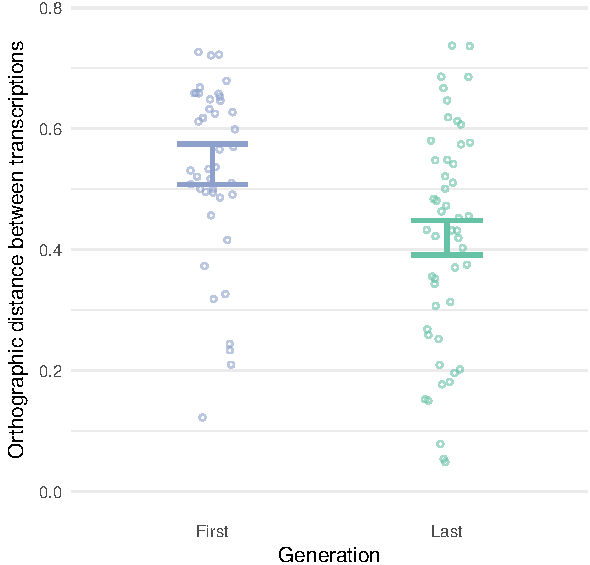
\includegraphics[width=8.0cm]{figs/fig3-1} 

}

\caption{Three types of matching questions depicted in relation to the original set of 16 seed sounds. For each question, participants listened to a sample imitation (orange circle) and had to guess which of 4 sound choices (green circles) they thought the person was trying to imitate. (Top) True seed questions contained the actual seed that generated the imitation in the choices, and the distrator seeds were sampled from different categories. (Middle) Category match questions also used distractor sounds from different categories but the correct seed was not the actual seed, but a different sound within the same category. (Bottom) Specific match questions pitted the actual seed against the other seeds within the same category.}\label{fig:fig3}
\end{figure}

\subsection{Results}\label{results-1}

Matching accuracy for all question types started above chance for the
first generation of imitations, \emph{b} = 1.65 (0.14) log-odds, odds =
0.50, \emph{z} = 11.58, \emph{p} \textless{} 0.001, and decreased
steadily over generations, \emph{b} = -0.16 (0.04) log-odds, \emph{z} =
-3.72, \emph{p} \textless{} 0.001. We tested whether this increase in
question difficulty was constant across the three types of questions or
if some question types became more difficult at later generations. In
particular we hypothesized that if the imitations were becoming more
like category labels as they were repeated, then performance on
questions where category information enabled a correct response would be
more resilient to transmissional decay.

The results are shown in Fig. 4. The first evidence in support of our
hypothesis comes in comparing performance on questions requiring a
category match to performance on questions where guessing correctly
required distinguishing the true seed from other sounds within the same
category. Performance decreased over generations more rapidly for these
specific match questions than for category match questions, \emph{b} =
-0.05 (0.02) log-odds, \emph{z} = -2.53, \emph{p} = 0.012, suggesting
that category information was more resistant to loss through
transmission.

One explanation for this result is that the specific match questions are
simply harder than the category match questions. However, performance
also decreased more rapidly for the easiest type of question where the
correct answer was the actual seed generating the imitation. The
advantage for having the true seed among the options decreased over
generations, \emph{b} = -0.07 (0.02) log-odds, \emph{z} = -2.83,
\emph{p} = 0.005. These results indicate that later generation
imitations were more likely to be recognized as identifiers of a
particular category than they were of particular exemplars within each
category.

\begin{figure}
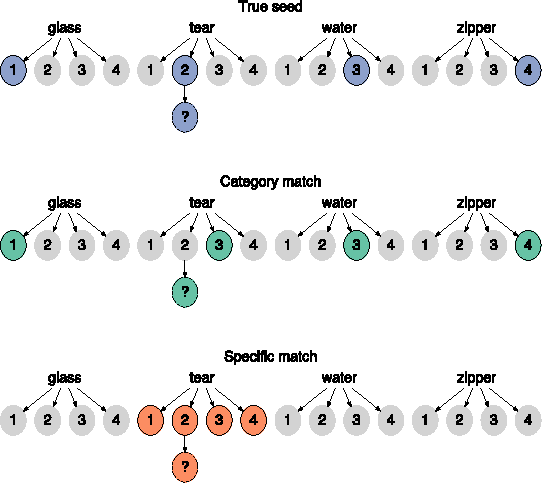
\includegraphics[width=8cm]{figs/fig4-1} \caption{Accuracy in matching imitations back to seed sounds. Performance is separated by question type based on the relationship between the imitation and the options in the question (see Fig. 3). Lines depict predictions from the generalized linear mixed effects model along with +/- 1 standard error of the model predictions.}\label{fig:fig4}
\end{figure}

\section{Experiment 3: Collecting transcriptions of
imitations}\label{experiment-3-collecting-transcriptions-of-imitations}

In addition to assessing stability in the acoustic properties of the
imitations, we also measured orthographic agreement and whether it too
changed over generations. We analyzed whether the imitations were also
becoming more stable in orthographic form.

\subsection{Methods}\label{methods-2}

\subsubsection{Materials}\label{materials-2}

We selected the first and final three imitations in each transmission
chain to be transcribed into English orthography.

\subsubsection{Procedure}\label{procedure-2}

Participants were instructed to write down what they heard as a word so
that the written word would sound as much like the message as possible.

\subsection{Results}\label{results-2}

We collected a total of 2182 or roughly 21 transcriptions per imitation.
All transcriptions containing actual English words were excluded from
analysis. Analyzing changes in orthographic agreement over generations
paralleled what was observed in the analysis of acoustic similarity:
Transcriptions from later generation imitations were more similar to one
another in terms of orthographic distance than transcriptions from
earlier generations, \emph{b} = -0.12 (0.03), \emph{t}(-3.6) = 3.05,
\emph{p} = 0.035 (Fig. 5). This result supports our hypothesis that the
imitations were becoming more stable in both acoustic and orthographic
forms.

\begin{figure}
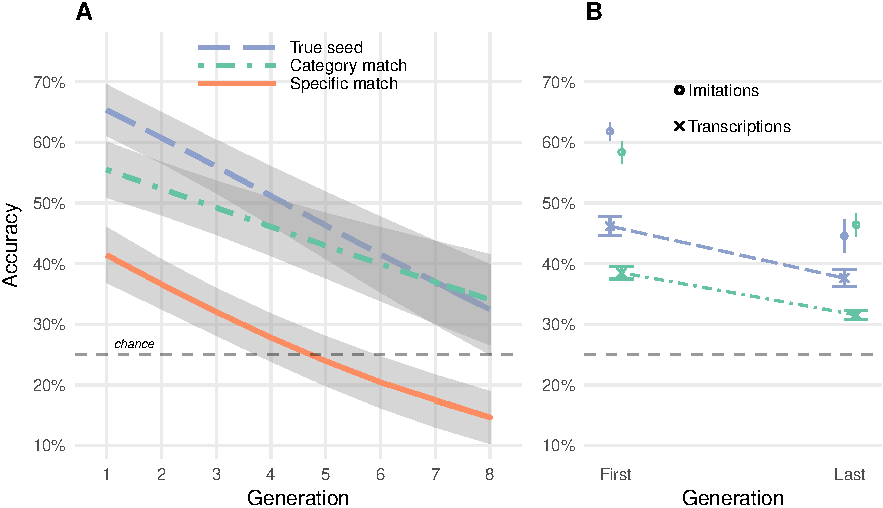
\includegraphics[width=8cm]{figs/fig5-1} \caption{Average orthographic distance among transcriptions of imitations taken from first and last generations. String distances were calculated between the most frequent transcription for each imitation compared to all others using the SequenceMatcher class available in the python standard library. Each point represents the average distance among all transcriptions for a single imitation. Error bars are +/- 1 standard error of the linear mixed effects model predictions.}\label{fig:fig5}
\end{figure}

\section{Experiment 4: Matching transcriptions to
seeds}\label{experiment-4-matching-transcriptions-to-seeds}

Experiment 4 tested whether the transcriptions obtained in Experiment 3
could be matched back to the original seed sounds. Although transcribing
the imitations stripped them of much of the analog signal in the
original sound, it still remained possible that what was transcribed
resembled the original sounds.

\subsection{Methods}\label{methods-3}

\subsubsection{Materials}\label{materials-3}

The top 4 most frequent transcriptions for each imitation transcribed in
Experiment 3 were tested in Experiment 4.

\subsubsection{Procedure}\label{procedure-3}

Participants completed a modified version of the 4AFC described in
Experiment 2. Instead of listening to imitations, participants now read
a transcription of an imitation, which they were told was an invented
word. They were instructed that the word was invented to describe one of
four presented sounds, and they had to guess which one.

\subsection{Results}\label{results-3}

Participants were able to guess the correct meaning of the transcribed
word above chance even after between 5 and 8 generations of repetition,
\emph{b} = 0.83 (0.13) log-odds, odds = -0.18, \emph{z} = 6.46, \emph{p}
\textless{} 0.001 (Fig. 6). This was true both for true seed questions,
\emph{b} = 0.75 (0.15) log-odds, odds = -0.28, \emph{z} = 4.87, \emph{p}
\textless{} 0.001, and for category match questions, \emph{b} = 1.02
(0.16) log-odds, odds = 0.02, \emph{z} = 6.39, \emph{p} \textless{}
0.001. The effect of generation did not vary across these question
types, \emph{b} = 0.05 (0.10) log-odds, \emph{z} = 0.47, \emph{p} =
0.637.

\begin{figure}
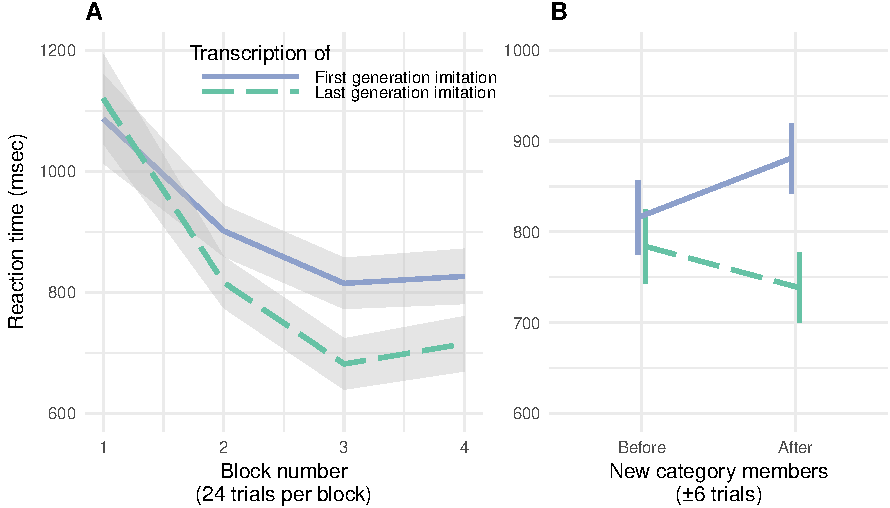
\includegraphics[width=8cm]{figs/fig6-1} \caption{Matching accuracy for transcriptions of imitations taken from first and last generations. True seed questions contained transcriptions of the actual seed generating the transcribed word. Category match questions contained transcriptions of imitations of other seeds from the same category.}\label{fig:fig6}
\end{figure}

\section{Experiment 5: Using transcriptions as category
labels}\label{experiment-5-using-transcriptions-as-category-labels}

In Experiment 5 we examined whether there was a learning advantage to
the more word-like imitations emerging through iterated repetition as
compared to direct imitations of the source of the sound. We
hypothesized that transcriptions of the more word-like forms emerging
through repeated imitation should be easier to generalize to new
category members than transcriptions from direct imitations.

\subsection{Methods}\label{methods-4}

\subsubsection{Materials}\label{materials-4}

To determine which transcriptions to test as category labels, we first
selected only those transcriptions which had above chance matching
performance when matching back to the original seeds. Then we excluded
transcriptions that had less than two unique characters or were over 10
characters long, and sampled from both first and last generation
imitations to reach a final set that controlled for overall matching
accuracy.

\subsubsection{Procedure}\label{procedure-4}

Participants learned, through trial-and-error, the names for four
different categories of sounds. On each trial participants listened to
one of the 16 environmental sounds used as seeds and then saw a novel
word--a transcription of one of the imitations. Participants responded
by pressing a green button if the label was the correct label and a red
button otherwise. They received accuracy feedback after each trial.

The experiment was divided into blocks so that participants had repeated
exposure to each sound and the novel labels multiple times within a
block. At the start of a new block, participants received four new
sounds from the same four categories (e.g., a new zipping sound, a new
water-splash sound, etc.) that they had not heard before, and had to
associate these sounds with the same novel labels from the previous
blocks. The extent to which their performance declined at the start of
each block serves as a measure of how well the label they associated
with the sound worked as a label for the category.

\subsection{Results}\label{results-4}

When participants had to generalize the meaning of the novel label to
new category members (new sounds), they were faster when the label came
from transcriptions of later generation imitations than from
transcriptions of first generation imitations, \emph{b} = -114.13
(52.06), \emph{t}(-2.2) = 39.92, \emph{p} = 0.034 (Fig. 7A). The effect
can be further localized within each block. Comparing RTs on the trials
leading up to a block transition and the trials immediately after the
block transition revealed a reliable interaction between block
transition and the generation of the transcribed label, \emph{b} =
-146.75 (65.47), \emph{t}(-2.2) = 1869.72, \emph{p} = 0.025 (Fig. 7B).
This suggests that in addition to becoming more stable both in terms of
acoustic and orthographic properties, imitations that have been more
repeated may also be easier to learn as category labels.

\begin{figure}
\includegraphics[width=8cm,height=10cm]{figs/fig7-1} \caption{(Top) RTs on correct trials by block, showing faster responses when learning category labels transcribed from last generation imitations. (Bottom) RTs on trials leading up to and immediately following the block transition where new category members are introduced.}\label{fig:fig7}
\end{figure}

\section{Discussion}\label{discussion}

We show that repeated imitation of an originally imitative vocalization
gradually becomes more word-like as it is transmitted along the chain of
a ``Telephone'' game. The first evidence provided showed that imitations
became more stable over generations of repetition, both in terms of
acoustic similarity as well as in orthographic agreement. But more than
just becoming more stable over generations, the imitations also become
more word-like in that served as more effective category labels.
Category information was more resilient to transmission decay than
specific information identifying a particular exemplar within a
category. This category information remained even when the imitations
were transcribed into lexical forms, as participants were able to guess
the categorical meaning of the word at above chance levels even after 8
generations of repetition. One such consequence of having words is that
they make categorization easier. In support of this conclusion, we found
that participants naive to the transmission chain experiment were faster
to learn category labels that had emerged through repeated imitation
than they learned from transcriptions of direct imitations of the
environmental sound, completing the transition from nonverbal imitation
to a fully lexicalized word form and demonstrating the impact of this
transition on communication.

One result that did not fit squarely with imitations becoming more
word-like is that with transcriptions, there was no difference over
generations between question types. If the results of matching
transcriptions back to seed sounds would have perfectly mirrored the
results of matching imitations back to seed sounds we would have
expected the difference between True seed questions and Category match
questions to decrease over generations. Instead we found a main effect
of question type. Although participants were able to match
transcriptions to categories of sounds even after 8 generations of
repetition, it was still easier for them to match a transcription to the
actual seed that generated the transcription.

Our study focused on the formation of onomatopoeia--sound-imitative
words--but in addition to onomatopoeia, many languages have semantically
rich systems of ideophones. These words comprise a grammatically and
phonologically distinct class of words that are used to express a
variety of sensory-rich meanings
\citep{Dingemanse:2012fc, Voeltz:2001vv}. Notably, these words are often
recognized by native speakers to be somehow imitative of their meaning.
For example, in Japanese, the word `koron' -- with a voiceless {[}k{]}
refers to a light object rolling once, the reduplicated `korokoro' to a
light object rolling repeatedly, and `gorogoro' -- with a voiced {[}g{]}
-- to a heavy object rolling repeatedly \citep{Imai:2014dea}. The
iconicity of ideophones was verified by an experiment that tested the
ability of naïve listeners to guess the meanings of words sampled from
five different languages \citep{Dingemanse:2016vd}. Although words for
sounds were guessed more accurately than the rest, listeners were better
than chance at guessing the synonyms of ideophones that expressed
meanings from all five semantic categories tested -- color/visual,
motion, shape, sound, and texture. In addition, laboratory experiments
show that people are able to generate imitative vocalizations for a
variety of non-sound concepts, and that these are also understandable to
naïve listeners \citep{Perlman:2015ip}. Thus vocal imitation has the
potential to play a role in word formation that extends beyond just the
imitation of sounds.

Our findings from an online game of Telephone suggest that the formation
of words from vocal imitation can be a simple process. The results show
how repeated imitation can create progressively more word-like forms
while retaining a resemblance to the original sound that motivated it.
This raises the possibility that onomatopoeic words can be created from
the repetition of one-shot vocal imitations of an original sound.

\bibliographystyle{apa}
\bibliography{telephone}

\end{document}
